\documentclass[11pt,twoside,a4paper]{article} % scrartcl

\usepackage{amsfonts}
\usepackage{amsmath}
\usepackage[hidelinks]{hyperref}
\usepackage[utf8]{inputenc}
\usepackage{listings} 
\lstset{language=ML}
\usepackage{proof}
\usepackage{qtree}
\usepackage{tikz}
\usepackage[normalem]{ulem}
\usetikzlibrary{arrows,calc,decorations.pathreplacing,matrix,shapes}

\bibliographystyle{alpha}

\newcommand{\nonterm}[1]{$\left<#1\right>$}
\newcommand{\alt}[0]{$|$}
\newcommand{\kw}[1]{{\bf \texttt{#1}}}
\newcommand{\mkw}[1]{{\bf \mathtt{#1}}}
\newcommand{\sym}[1]{\texttt{#1}}
\newcommand{\msym}[1]{\mathtt{#1}}
\newcommand{\centeredtab}[1]{\begin{center}\parbox{0cm}{\begin{tabbing}#1\end{tabbing}}\end{center}}
\newcommand{\msout}[1]{\text{\sout{\ensuremath{#1}}}}
\def\squareborder#1{\tikz\node[draw]{#1};} 

\pgfarrowsdeclarecombine{twostealth}{twostealth}%
{stealth}{stealth}{stealth}{stealth}

\begin{document}

\title{Introduction to Lambda Calculus}
%\subtitle{notes} 
\author{Maciek Makowski (\texttt{@mmakowski})}
\maketitle

\section{Motivation}

Software is pervasive in the modern world and has influence over many aspects 
of our lives. In some cases, such as avionics or medical equipment control, 
human life depends on the correctness of software. Yet, high profile cases of 
bugs\footnote{Infamous historical examples include Mars Climate 
Orbiter's inconsistent usage of units of measurement\cite{mco} and Therac-25 
radiation therapy overdoses\cite{therac25}. Recent faults such as
security-related Apple goto fail\cite{cve141266} and OpenSSL Heartbleed
bug\cite{cve140160},
while not life-threatening, had wide-ranging implications for the security of
e-commerce and privacy of internet users.} do not inspire confidence in the 
state of software engineering. 

The "software crisis" is a phenomenon recognised 
by practitioners of the field. Several ways of addressing the reliability issue 
have been proposed: from reliance on programmer's 
discipline\cite{cleancode}\cite{securecoding}, through tools that
perform post-hoc validation of programs to ensure they do not contain suspicious
coding patterns\cite{raf04}, to languages 
that restrict valid programs to ones whose properties can be formally proven. 
The latter approach relies on a body of 
theoretical knowledge that can appear intimidating. It turns out, 
however, that much of the required insight is built on systematic extensions of 
a very simple formal system -- the lambda calculus. 

While understanding of the basics of lambda calculus will not immediately 
make us experts in formal methods, it is a gateway to the world of software
engineering tools whose roots are in logic, mathematics and formal reasoning.
Lambda calculus makes the task of learning advanced programming trechniques
manageable by providing a simple framework within which programming constructs
can be understood.

\section{Syntax}

Given a set $\mathbb{X}$ of variables, terms of lambda calculus are generated by the 
following grammar:
\begin{tabbing}
\nonterm{term} \= ::=  \= $x$~~~~~~~~~~~~~~~~~~~~~~~~~~~~ \= (variable)    \\
               \> \alt \> ($\lambda x.$\nonterm{term})    \> (abstraction) \\
               \> \alt \> (\nonterm{term} \nonterm{term}) \> (application) 
\end{tabbing}
where $x\in \mathbb{X}$. Notational convention is that application binds to the left, the 
full-stop can be treated as an opening parenthesis that extends until the end of 
the sub-term and redundant parentheses are omitted. 

\paragraph{Example:} shown below are sample lambda terms, on the left
as they are typically written, on the right actual ASTs:
\begin{tabbing}
$v_1$~~~~~~~~~~~~~~~~~~~~~~~~~~~~~~~~~~~~~~ \= \Tree [.{var $v_1$} ]           \\
\noindent\rule{12.5cm}{0.4pt}                                                  \\
$x\ y\ z$                                   \> \Tree [.app [.app {var $x$} 
{var $y$} ] {var $z$} ]                                                        \\
\noindent\rule{12.5cm}{0.4pt}                                                  \\
$(\lambda a.\lambda b.a)\ c\ (\lambda b.b)$ \> \Tree [.app [.app [.{abs $a$} 
[.{abs $b$} {var $a$} ] ] {var $c$} ] [.{abs $b$} {var $b$} ] ]                \\
\end{tabbing}
Within a term, occurrences of variables that are not bound by enclosing abstraction
-- i.e. where the variable name does not appear in any abs node on the path to the 
root of the AST -- are called \emph{free}. 

\paragraph{Example:} free occurrences have been marked in the sample term
below:
\begin{tabbing}
~~~~~~~~~~~~~~~~~~~~~~~~~~~~~~~~~~ \= ~~~~~~~~~~~~~~~~~~~~~~~~~~~~~~~~~~~~ \\
$(\lambda a.\underline{b}\ a)\ \underline{c}\ (\lambda b.b)$ \> 
\Tree [.app [.app [.{abs $a$} [.app \squareborder{var $b$} {var $a$} ] ] 
\squareborder{var $c$} ] [.{abs $b$} {var $b$} ] ]            \\
\end{tabbing}
Note that the same variable name might have both bound and free occurrences
within a term, as in the second example. Terms with no free occurrences are known 
as \emph{closed terms}, or \emph{combinators}.

\paragraph{Summary:} we have defined what lambda terms look like. The grammar 
has three productions -- variable, abstraction and application -- and generates 
abstract syntax trees.

\section{Rewriting Rules}

Lambda terms are not of much use without some operations that can be performed
on them. Two\footnote{The third frequently applied operation is introduction/removal 
of abstraction ($\eta$-conversion): $\lambda x.M\,x\longleftrightarrow_\eta M$ for 
any term $M$. We will not require it in this presentation of lambda calculus.} 
operations we will use going forward are presented below.

\subsection{Renaming of bound variables}

Intuitively, $\lambda x.x$ is similar to $\lambda y.y$ -- the "shape" of these
two terms is the same, they differ only in the choice of variable used. In 
practice we will often want to identify terms of the same structure. 
This intuitive similarity is captured by an operation called 
\emph{$\alpha$-conversion} that consistently renames variables. While the
operation appears trivial, there are subtleties around bound vs. free
variables -- for instance, nested abstractions can use the same variable name
-- but these difficulties manifest themselves mostly in the
implementation\footnote{For that reason a convenient way to represent 
lambda terms when implementing evaluation is positional (de Bruijn) encoding
which replaces variable names with numerical index of the lambda that binds given 
variable occurrence. For example, de Bruijn representation of 
$\lambda a.\lambda b.a\ b\ c$  would be $\lambda.\lambda.1\ 0\ 2$ under naming 
context $\{c\mapsto 2\}$.  The naming context is required to map free variables 
to indices.}, so we will not worry about them in this presentation. The intuition 
about variable renaming is correct in most cases we are interested in. In 
particular, we can assume that all the variables in the terms we are working 
with have been chosen so that they are distinct. It is always possible to 
$\alpha$-convert any term so that this is true.
\paragraph{Example:} $(\lambda x.x\,y)\ (\lambda x.x)\longleftrightarrow_\alpha(\lambda
a.a\,y)\ (\lambda b.b)$

\subsection{Removal of abstraction under application}\label{beta-reduction}

The basic operation that modifies the structure of the term is
\emph{$\beta$-reduction}. It can be applied to every term or sub-term that is
an application whose left-hand side is an abstraction:
\begin{align*}
(\lambda x.M)\ N\longrightarrow_\beta M[x/N]
\end{align*}
where $M[x/N]$ is term $M$ in which all free occurrences of $x$ have been
replaced by term $N$.

\paragraph{Example:} $(\lambda x.x\,y)\ (\lambda z.z)\longrightarrow_\beta
(\lambda z.z)\ y\longrightarrow_\beta y$\\
In the first reduction, $\lambda x.$ is eliminated by substituting $\lambda z.z$ 
for $x$, in the second, $\lambda z.$ is eliminated by substituting $y$ for $z$.

This is the key operation of lambda calculus, as it represents a
\emph{computation}. It allows us to view a lambda term as a program that can be
evaluated to a final value (i.e. a term that cannot be further reduced). That
final value is called a \emph{normal form} of a term.

An application that can be $\beta$-reduced is called a \emph{redex}. There can
be multiple redexes in a given term:
\begin{center}
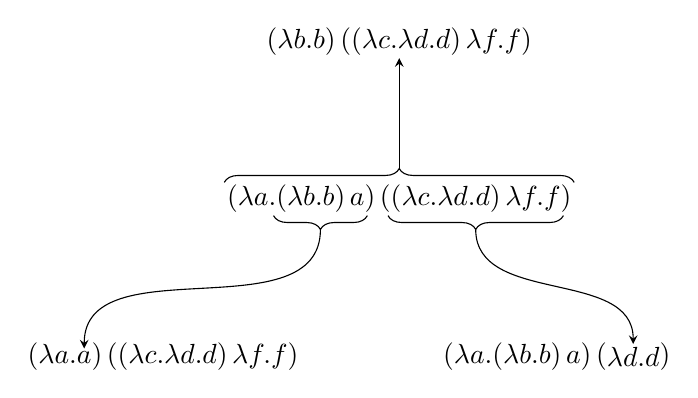
\begin{tikzpicture}[every node/.style={inner sep=0,outer sep=1}]
    \node[matrix](s1) at (3,0) {
        \node     {$(\lambda a.$}; &
        \node(s2) {$(\lambda b.b)\,a$}; &
        \node     {$)\,($}; &
        \node(s3) {$(\lambda c.\lambda d.d)\,\lambda f.f$}; &
        \node     {$)$}; \\
    };
    \node(d1) at (3,2) {$(\lambda b.b)\,((\lambda c.\lambda d.d)\,\lambda f.f)$};
    \node[matrix] at (0,-2){
        \node                   {$(\lambda a.$}; &
        \node(d2) at (0, -0.01) {$a$}; &
        \node                   {$)\,((\lambda c.\lambda d.d)\,\lambda f.f)$}; \\
    };
    \node[matrix] at (5,-2){
        \node     {$(\lambda a.(\lambda b.b)\,a)\,($}; &
        \node(d3) {$\lambda d.d$}; &
        \node     {$)$}; \\
    };
    \draw[decorate,decoration={brace,amplitude=5pt}]
    (s1.north west)--(s1.north east);
    \draw[-stealth] ($(s1.north)+(0,5pt)$) to node[right,midway]{}(d1);
    \draw[decorate,decoration={brace,mirror,amplitude=5pt}]
    (s2.south west)--(s2.south east);
    \draw[-stealth] ($(s2.south)+(0,-5pt)$) to [out=-90,in=90] node{}(d2);
    \draw[decorate,decoration={brace,mirror,amplitude=5pt}]
    (s3.south west)--(s3.south east);
    \draw[-stealth] ($(s3.south)+(0,-5pt)$) to [out=-90,in=90] node{}(d3);
\end{tikzpicture}
\end{center}

The choice of the redex to be reduced next is up to us. Prescribing which redex
should be chosen gives rise to a reduction strategy. For example:
\begin{itemize}
\item restricting reduction to only the redexes that are not under abstraction
and always starting with the innermost redex is \emph{call-by-value} strategy;
\item similarly restricting reduction to redexes that are not under
abstraction, but starting with outermost redex is \emph{call-by-name}\footnote{
Scala uses call-by-value evaluation strategy everywhere except for by-name
function arguments (\texttt{arg: => T}) where call-by-name is used}.
\end{itemize}
Different evaluation strategies can stop at different terms; for example, if we
use call-by-value then the chain of reductions will stop once there are no more
redexes outside of abstractions. A more permissive strategy would allow the
reductions to continue with those redexes under abstractions. Perhaps more
interestingly, there are terms which loop forever under some evaluation
strategies but reduce to a normal form under others. That said, unrestricted 
$\beta$-reduction is \emph{confluent}: if a term $S$ can be reduced in two 
different ways, producing terms $T$ and $U$, then $T$ and $U$ can both be reduced 
to some common term $V$:
\begin{center}
\begin{tikzpicture}[->,>=twostealth,node distance=2cm]
    \node(S) {$S$};
    \node(T) [below left of=S] {$T$};
    \node(U) [below right of=S] {$U$};
    \node(V) [below left of=U] {$V$};
    \draw (S) -- (T);
    \draw (S) -- (U);
    \draw[densely dotted] (T) -- (V);
    \draw[densely dotted] (U) -- (V);
\end{tikzpicture}
\end{center}
This is formalised as \emph{Church-Rosser theorem} and is an
important result: it allows us to disregard the order of reductions when
considering the semantics of a lambda term. Specifically, it justifies the
interchangeability of lazy and eager evaluation.

Does a chain of $\beta$-reductions terminate for every term? No; take as an example 
$(\lambda x.xx) (\lambda x.xx)$. This term, called $\Omega$, $\beta$-reduces to 
itself.

\paragraph{Summary:} lambda-terms can be syntactically transformed according to 
two rules: $\alpha$-conversion, which renames the variables, and $\beta$-reduction,
which "applies" one term to another.

\section{Mathematical Interpretation}

So far we have discussed the syntax of lambda calculus without any mention of
its semantics. The purpose of this restriction was to stress that all the
constructs we will be building are defined as manipulation of term trees,
and any meaning we might associate with them is secondary. That said,
the upcoming sections will be much easier to understand with a mental model of
what a lambda term represents. It perhaps comes as no surprise that a lambda
abstraction can be interpreted as an anonymous function. 

\paragraph{Example:} in common mathematical notation we would write 
\begin{align*}
f(x)=3*x+2
\end{align*}
to describe a linear function of $x$. The same function can be represented by 
lambda term 
\begin{align*}
\lambda x.+\,(*\,3\,x)\,2
\end{align*}
where $*$ and $+$ are predefined binary 
functions that respectively multiply and add numbers and are written in prefix
notation due to lambda calculus syntactic rules.
\\\\
Lambda application is then simply application of the function represented by
the first subterm to the argument represented by the second subterm. In this
model, $\beta$-reduction is a method of function evaluation.

\paragraph{Summary:} lambda abstractions can be interpreted as mathematical 
functions.

\section{Programming}

We claimed that a lambda term can be treated as a computer program. To substantiate 
this, let us see how familiar elements of programming languages can be represented 
in lambda calculus\footnote{One definition of functional programming is 
"programming with mathematical functions". By presenting how to program with
lambda terms, which, we argued, represent such functions, we will demonstrate
the basics of functional programming.}.

\subsection{Conditionals}

Choice of execution path to follow is a fundamental building block of most
algorithms. It is usually represented as 
\begin{center}
\kw{if} $C$ \kw{then} $T$ \kw{else} $F$
\end{center}
where $C$ evaluates to either \sym{true} or \sym{false}, where \sym{true} and 
\sym{false} are some specific values chosen by us beforehand. If $C$ evaluates 
to \sym{true} then the whole conditional expression evaluates to the result of 
$T$, otherwise it evaluates to the result of $F$. To start with, let us choose 
some lambda-terms that will represent \sym{true} and \sym{false}\footnote{Note
that the syntax $\msym{name} = T$ is not part of lambda calculus, it is just
our way of giving meaningful names to terms. We can think of it as a
preprocessor macro.}:
\begin{align*}
\msym{true}  &= \lambda t.\lambda f.t \\
\msym{false} &= \lambda t.\lambda f.f
\end{align*}
With these in place, the conditional expression can be written as
\begin{align*}
\msym{test} &= \lambda c.\lambda t.\lambda f.c\,t\,f \\
\mkw{if}\,C\,\mkw{then}\,T\,\mkw{else}\,F &= \msym{test}\,C\,T\,F
\end{align*}
It is easy to see that indeed, if $c$ is \sym{true} then $\beta$-reduction of
$c\,t\,f$ will yield $t$ and if it is \sym{false} then it will reduce to $f$.

\subsection{Numbers}

Another primitive essential in programming as we know it are numbers. After
Peano, we can specify the set of natural numbers by means of a chosen value
\sym{0} and a function \sym{succ} that maps every natural number to
its successor. In lambda calculus these can be encoded as follows:
\begin{align*}
\msym{0}    &= \lambda s.\lambda z.z \\
\msym{succ} &= \lambda n.\lambda s.\lambda z.s\,(n\,s\,z)
\end{align*}
This is what terms representing numbers look like with these 
definitions\footnote{Seeing how Peano arithmetic can be defined in lambda calculus,
and drawing parallels with Zermelo-Fraenkel set-theoretical model of
natural numbers and the build-out of other mathematical constructs on this
basis, one could ask: can untyped lambda calculus be treated as a foundational
theory in which all known mathematical concepts can be stated? Alonso Church had 
that in mind when he conceived lambda calculus, but it was soon proven by his 
studens, Kleene and Rosser\cite{wkrp}, that in fact the calculus as we present it here is 
inconsistent, i.e. any proposition can be proven in it.}:
\centeredtab{
\sym{0} \= $=$ \= ~~~~~~~~~    \= ~~~ \= $\lambda s.\lambda z.z$    \\
\sym{1} \> $=$ \> \sym{succ 0} \> $=$ \> $\lambda s.\lambda z.s\,z$ \\
\sym{2} \> $=$ \> \sym{succ 1} \> $=$ \> $\lambda s.\lambda z.s\,(s\,z)$ \\
\sym{3} \> $=$ \> \sym{succ 2} \> $=$ \> $\lambda s.\lambda z.s\,(s\,(s\,z))$ \\
$\vdots$ \\
\sym{n} \> $=$ \> \> \> $\lambda s.\lambda z\underbrace{s\,(\dots s\,(s}_n\,z)\dots)$
}
Definition of arithmetics in this representation is reasonably straightforward
in case of addition and multiplication:
\begin{align*}
\msym{plus}  &= \lambda m.\lambda n.\lambda s. \lambda z.m\ s\ (n\ s\ z) \\
\msym{times} &= \lambda m.\lambda n.m\ (\msym{plus}\ n)\ \msym{0}
\end{align*}
Subtraction, however, turns out to be much more tricky to define\footnote{If
you attempt to do this as an exercise you might want to start with defining a
function \sym{pred} -- the inverse of \sym{succ}.}.

\subsection{Repeated Calculation}

With numbers and conditionals in place, our language is still severely
restricted. For example, how would we write a factorial function? As a
reminder, the mathematical definition of factorial is
\begin{align*}
n!=\begin{cases}
    1 & \text{if $n=0$},\\
    n*(n-1)! & \text{otherwise}.
  \end{cases}
\end{align*}
Implementation in a typical programming language involves either a recursion or
a loop, neither of which is directly supported by lambda calculus. A way to
deal with this is \emph{fixed point operator}:
\begin{align*}
\msym{Y}=\lambda f.(\lambda x.f\,(x\,x))\,(\lambda x.f\,(x\,x))
\end{align*}
How does that help? Intuitively, we can construct a function parameterised by a 
function, then use \sym{Y} to feed the function into itself. For example factorial
can be defined as follows\footnote{Note that this definition is expressed 
entirely in lambda calculus. We have
previously shown how to encode \sym{if-then-else}, \sym{times} and numbers,
\sym{pred} and \sym{eq} can also be encoded with a little bit more machinery
than what we managed to show in this short introduction -- see e.g. \cite{TAPL} for 
full details.}:
\begin{align*}
\msym{g} &= \lambda f.\lambda
n.\mkw{if}\ \msym{eq}\ n\ \msym{0}\ \mkw{then}\ \msym{1}\ \mkw{else}\ (\msym{times}\ \msym{n}\,(f\,(\msym{pred}\ \msym{n}))) \\
\msym{factorial} &= \msym{Y}\ \msym{g}
\end{align*}
To illustrate the working of \sym{Y} let let us follow a single stage of evaluation
(single recursive descent) of \sym{factorial} \sym{3}:
\\\\
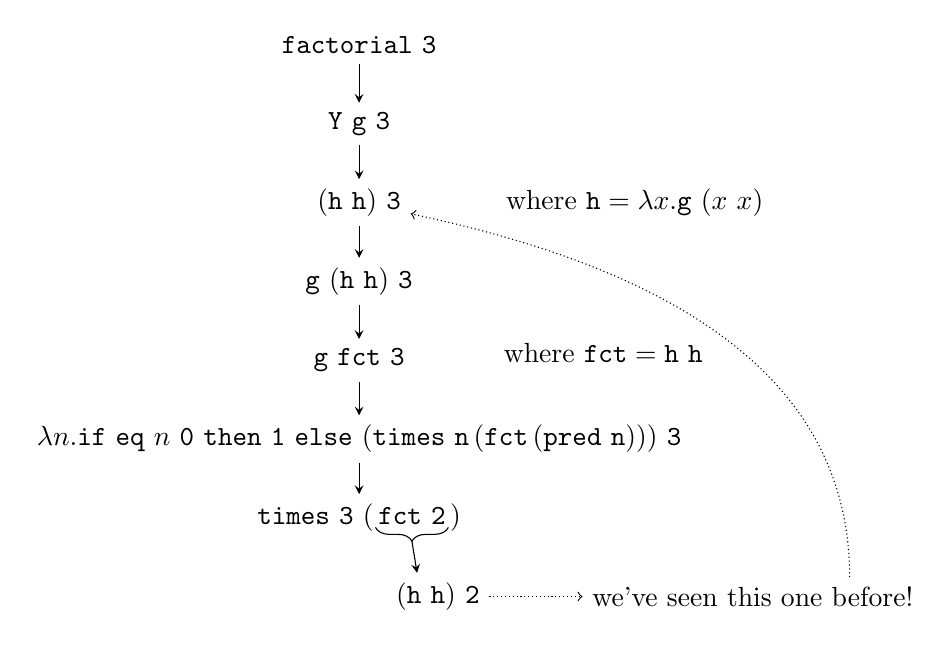
\begin{tikzpicture}
    \node(e1) at (0,10) {\sym{factorial} \sym{3}};
    \node(e2) at (0,9)  {\sym{Y} \sym{g} \sym{3}};
    \node(e3) at (0,8)  {$(\msym{h}\ \msym{h})\ \msym{3}$}; 
    \node(exp3) at (3.5,8) {where $\msym{h}=\lambda x.\msym{g}\ (x\ x)$};
    \node(e4) at (0,7)  {$\msym{g}\ (\msym{h}\ \msym{h})\ \msym{3}$};
    \node(e41) at (0,6)  {$\msym{g}\ \msym{fct}\ \msym{3}$};
    \node(exp41) at (3.1,6.1) {where $\msym{fct}=\msym{h}\ \msym{h}$};
    \node(e5) at (0,5)  {
        $\lambda n.\mkw{if}\ \msym{eq}\ n\ \msym{0}\ \mkw{then}\ \msym{1}\\\ \mkw{else}\ (\msym{times}\ \msym{n}\,(\msym{fct}\,(\msym{pred}\ \msym{n})))\ \msym{3}$
    };
    \node[matrix](me6) at (0,4) {
        \node[style={inner sep=0,outer sep=1}]     { $\msym{times}\ \msym{3}\ (\,$ }; &
        \node[style={inner sep=0,outer sep=1}](e6) at (0, 0.02) { $\msym{fct}\ \msym{2}$ }; &
        \node[style={inner sep=0,outer sep=1}]     { $\,)$ }; \\
    };
    \node(e7) at (1,3)  {$(\msym{h}\ \msym{h})\ \msym{2}$};
    \node(conc) at (5,3) {we've seen this one before!};
    \path[-stealth]
      (e1) edge (e2)
      (e2) edge (e3)
      (e3) edge (e4)
      (e4) edge (e41)
      (e41) edge (e5)
      (e5) edge (me6)
      ;
    \draw[decorate,decoration={brace,mirror,amplitude=5pt}] (e6.south west)--(e6.south east);
    \draw[-stealth] ($(e6.south)+(0,-5pt)$) to ($(e7.north)-(7.5pt,0)$);
    \draw[densely dotted,->] (e7) to (conc);
    \draw[densely dotted,->] ($(conc.north)+(35pt,0)$) to[out=90,in=-12] (e3);
\end{tikzpicture}
\\\\
In general, a recursive function \sym{f}, that in a language that supports
direct recursion would be defined as
\begin{align*}
\mkw{fun}\ \msym{f} = M(\msym{f})
\end{align*}
where $M(\msym{f})$ is the body of the function that contains reference to \sym{f}, 
in lambda calculus can be defined as
\begin{align*}
\msym{f} = \msym{Y}\ (\lambda f.M(f))
\end{align*}

\paragraph{Summary:} we can encode common programming constructs such as
conditionals, numbers and recursion\footnote{We have only shown how to encode 
a function that invokes itself recursively. Mutual recursion, i.e. a set of 
functions where each function can invoke each other in cyclic fashion can also 
be represented. We can construct a record of functions -- at this point it 
might come as no surprise that a record can be encoded as a lambda abstraction
-- and apply \kw{Y} to that record. See \cite{TAPL} for details.} as lambda 
terms.

\section{Types}\label{types}

If $\mathbb{T}$ is the set of type variables then the grammar of types is:
\begin{tabbing}
\nonterm{type} \= ::=  \= $\sigma$                                      \\
               \> \alt \> (\nonterm{type} $\rightarrow$ \nonterm{type}) 
\end{tabbing}
where $\sigma\in\mathbb{T}$. Notational convention is that arrow binds to the
right, so we can write $\sigma\rightarrow\tau\rightarrow\rho$ instead of 
$(\sigma\rightarrow (\tau\rightarrow\rho))$.

Lambda terms can be assigned types by following the structure of the AST. We 
start with the leaves of the tree, i.e. variables, and make note of assumptions 
about their types; for example, $x:\sigma$ means that we assume variable $x$ to
have type $\sigma$. We then proceed up the tree, applying the following two
rules to inner nodes:
\centeredtab{
\infer{M\,N:\tau}{M:\sigma\rightarrow\tau & & N:\sigma}~~~~~~~~~~~           \= (application) \\\\\\ 
\infer{\lambda x.M:\sigma\rightarrow\tau}{\infer*{M:\tau}{\msout{x:\sigma}}} \> (abstraction)
}
In abstraction rule, we need to first make an assumption about the type of 
variable $x$ that might occur free in term $M$. Once we establish the type 
of $M$ to be $\tau$ based on this assumption, we use the assumed type as the 
type of argument of the abstraction, at which point the assumption is no longer 
needed -- hence the crossing out.

As we proceed applying the rules, we might need to refine the
assumptions. If we initially assumed $x:\sigma$ and $f:\tau$ but then come
across application $f\,x$ then we know from the rule for application that the
type of $f$ must be an arrow type, so we have to refine the assumption to
$f:\sigma\rightarrow\rho$.

\paragraph{Example:} what is the type of $\lambda f.\lambda x.f(f\,x)$?
\begin{align*}
\infer[(abs)]{\lambda f.\lambda x.f(f\,x):(\sigma\rightarrow\sigma)\rightarrow\sigma\rightarrow\sigma}{
  \infer[(abs)]{\lambda x.f(f\,x):\sigma\rightarrow\sigma}{
    \infer[(app)]{f(f\,x):\sigma}{\msout{f:\sigma\rightarrow\sigma} &
      \infer[(app)]{f\,x:\sigma}{\msout{f:\sigma\rightarrow\sigma} & \msout{x:\sigma}}
    }
  }
}
\end{align*}
The first use of abstraction rule eliminated the need for $x:\sigma$
assumption, the second eliminated $f:\sigma\rightarrow\sigma$.
\\

We write $\Gamma\vdash M:\sigma$ to state that there exists a derivation with 
the set of assumptions (context) $\Gamma$ that assigns type $\sigma$ to term $M$. 
Notational convetion is that when the $\Gamma$ is empty it
can be omitted altogether, so for the example above we can write
$\vdash \lambda f.\lambda
x.f(f\,x):(\sigma\rightarrow\sigma)\rightarrow\sigma\rightarrow\sigma$\footnote{This
way of inferring types of terms has been introduced by Curry. An alternative
system, by Church, requires explicit type declarations. These two calculi
differ in some of their properties, but the type derivations in both are essentially
equivalent\cite{su99}.}.

Lambda calculus whose set of terms is restricted to terms that can be
assigned types according to the rules above is called \emph{simply-typed lambda
calculus} and denoted by $\lambda_\rightarrow$. The typing restriction is
severe: it only admits terms whose $\beta$-reduction terminates with a term that 
cannot be reduced further\footnote{This property is called \emph{strong normalisation}.}. 
For example, recursion
cannot be implemented in this calculus.\footnote{This restriction can be seen as a good
thing, since it eliminates a class of terms which we might not want to write, for
example those that loop indefinitely, or as a bad thing, since it prevents us
from writing useful functions such as the Fibonacci sequence. In practice this
is the tension that programming language designers grapple with: provide a type
system that eliminates as many undesirable programs as possible while
eliminating as few desirable programs as possible.}

\paragraph{Summary:} lambda terms can be assigned types, which are built from
type variables and arrows. If we insist that only terms that have a type are 
valid, we place limits on how the reduction of such terms can behave.

\section{Curry-Howard Correspondence}

In classical propositional logic every formula is either true or false.
\emph{Intuitionistic logic} is an alternative system, where a statement is true
if it can be proven constructively\footnote{For this reason intuitionistic logic 
is also known as \emph{constructive logic}.} and false if a contradiction can
be inferred from it. If neither of these is the case the truth of the statement
remains unknown. A consequence of intuitionistic approach is that some 
of classical tautologies, such as the law of excluded middle, $p\vee\neg p$, cannot 
be proven.

Proofs in intuitionistic logic are trees with the formula to be proven in the root,
axioms in the leaves and inner nodes containig formulae that can be inferred
from children using a set of prescribed rules. As such, these proofs directly
correspond to computations. As we argued in \ref{beta-reduction}, so do lambda
terms. Furthermore, types of simply-typed lambda calculus can be read as statements 
in the fragment of intuitionsitic logic that uses implication ($\rightarrow$) as 
the only logical connective. It turns out that the terms in this calculus can
be interpreted as proofs of the propositions represented by their types. For a
hint of how such proofs may look see the derivation tree for
$\lambda f.\lambda x.f(f\,x):(\sigma\rightarrow\sigma)\rightarrow\sigma\rightarrow\sigma$
in section \ref{types}.\footnote{In fact, the typing rules for application and
abstraction directly correspond to two basic inference rules in propositional
logic: implication elimination (\textit{Modus Ponens}) and implication introduction.}

The Curry-Howard correspondence does not end on $\lambda_\rightarrow$. It can
be extended to a huge variety of type systems and logics and this fact has been 
exploited to transfer results between the fields of logic and computer 
science\footnote{For an example of practical application of Curry-Howard correspondence 
see \cite{s11}.}.

\section{More Types}

Simply-typed lambda calculus discussed in section \ref{types} was very restrictive. More 
elaborate calculi build on top of simply-typed lambda calculus by providing
extensions that allow typing of more terms. The diagram below shows some of the 
extensions.
\begin{center}
\begin{tikzpicture}
  \matrix(m)[matrix of math nodes, row sep=3em, column sep=3em]{
                 & F^\omega_{<:}       &                     & \lambda\omega             &            & \lambda P\omega      \\
    F_{<:}       &                     & \lambda 2           &                           & \lambda P2 &                      \\
                 &                     &                     & \lambda\underline{\omega} &            & \lambda P\underline{\omega} \\
    \lambda_{<:} &                     & \lambda_\rightarrow &                           & \lambda P  &                      \\
  };
  \path[-stealth]
    (m-4-3) edge (m-2-3) edge (m-4-5) edge [densely dotted] (m-3-4)
    (m-3-4) edge [densely dotted] (m-1-4) edge [densely dotted] (m-3-6)
    (m-2-3) edge (m-1-4) edge [-,line width=6pt,draw=white] (m-2-5) edge (m-2-5)
    (m-4-5) edge (m-3-6) edge [-,line width=6pt,draw=white] (m-2-5) edge (m-2-5)
    (m-1-4) edge (m-1-6)
    (m-2-5) edge (m-1-6)
    (m-3-6) edge (m-1-6)
    % end of cube edges
    (m-4-3) edge (m-4-1)
    (m-4-1) edge (m-2-1)
    (m-2-3) edge (m-2-1)
    (m-2-1) edge (m-1-2)
    (m-1-4) edge (m-1-2);
\end{tikzpicture}
\end{center}
Three of the direct extensions of simply-typed lambda calculus -- $\lambda_\rightarrow$ in the
diagram -- are obtained by adding various forms of dependencies between types
and terms:
\begin{itemize}
\item $\lambda 2$, also known as \emph{System F}; adds terms depending on
types, i.e. \emph{polymorphism}
\item $\lambda\underline{\omega}$; adds types depending on types, i.e. \emph{type
operators}
\item $\lambda P$; adds types depending on terms, i.e. \emph{dependent types}
\end{itemize}
These extensions can be combined further into more powerful calculi. The eight
calculi based on simple types and the three extensions mentioned form the
\emph{lambda cube}\cite{b91}.

In addition, subtyping ($<:$) can be added to $\lambda_\rightarrow$, and a
combination of this calculus with extensions of System F provides calculi in
which object orientation can be modelled.

\section{Combinatory Logic}

Let us define the following two combinators:
\begin{align*}
\msym{K} &= \lambda x.\lambda y.x \\
\msym{S} &= \lambda x.\lambda y.\lambda z.x z (y z)
\end{align*}
First, notice that the identity function, $\lambda x.x$, can be expressed as 
$\msym{S}\,\msym{K}\,\msym{K}$. We will denote this as $I$. It turns out that any 
lambda term can be expressed as a sequence of applications 
of \sym{S} and \sym{K}\footnote{More precisely, for any lambda term $T$ there exists an
expression $U$ that consist only of application of \sym{S} and \sym{K} that is 
\textit{extensionally equivalent} to $T$, i.e. for any term $V$, application $TV$ can be
$\beta$-reduced to some term to which $UV$ can also be $\beta$-reduced.}. 
We can define a translation function $T$ as follows:
\begin{align*}
T[\msym{K}]    &= \msym{K} \\
T[\msym{S}]    &= \msym{S} \\
T[x]           &= x \\
T[(E_1\,E_2)]  &= (T[E1]\,T[E2]) \\
T[\lambda x.E] &= \begin{cases}
    \text{if $x$ occurs free in $E$:} & \begin{cases}
        \text{if $E=x$:}             & \msym{I},\\
        \text{if $E=\lambda y.E_1$:} & T[\lambda x.T[\lambda y.E_1]], \\
        \text{if $E=(E_1\,E_2)$:}    & (\msym{S}\,T[\lambda x.E_1]\,T[\lambda x.E_2
        ],
    \end{cases} \\
    \text{otherwise:} & (\msym{K}\,T[E]).
  \end{cases}
\end{align*}

\paragraph{Example:}
\begin{align*}
T[\lambda x.\lambda y.yx] &= T[\lambda x.T[\lambda y.yx]] \\
                          &= T[\lambda x.\msym{s}\,T[\lambda y.y]\,T[\lambda y.x]]
                          \\
                          &= T[\lambda x.\msym{S}\,\msym{I}\,(\msym{K}\,x)] \\
                          &= \msym{S}\,T[\lambda x.\msym{S}\,\msym{I}]\,T[
                          \lambda x.\msym{K}\,x] \\
                          &= \msym{S}\,(\msym{K}\,T[\msym{S}\,\msym{I}])\,(\msym
                          {S}\,T[\lambda x.\msym{K}]\,T[\lambda x.x]) \\
                          &= \msym{S}\,(\msym{K}\,(\msym{S}\,\msym{I}))\,(\msym{
                          S}\,(\msym{K}\,\msym{K})\,\msym{I})
\end{align*}

The fact that any computable function can be expressed using only these two
combinators is quite interesting in its own right, but we can do even better. 
Consider:
\begin{align*}
\msym{X} &= \lambda x.x\,\msym{S}\,\msym{K}
\end{align*}
Now, we can express \sym{S} and \sym{K} using just \sym{X}:
\begin{align*}
\msym{K} &= \msym{X}\,(\msym{X}\,(\msym{X}\,\msym{X})) \\
\msym{S} &= \msym{X}\,(\msym{X}\,(\msym{X}\,(\msym{X}\,\msym{X})))
\end{align*}
That is, all computable functions can be expressed just as some sequence of
applications of a single combinator.


\section{Further Reading}

A direct inspiration for this talk was the presentation of lambda calculus in
\cite{TAPL}. The book is very well written and builds a sophisticated type
system in easy to follow steps, starting from untyped lambda calculus. 

For a succinct but rigorous introduction to lambda calculus see \cite{bb00}.
\cite{su99} contains a complete formal introduction to lambda calculus and an
extensive material on Curry-Howard correspondence.

\begin{thebibliography}{9}
\bibitem[TAPL]{TAPL} Benjamin C. Pierce, \emph{Types and Programming Languages},
\url{http://www.cis.upenn.edu/~bcpierce/tapl/}
\bibitem[SU99]{su99} Morten Heine B. Sørensen, Paweł Urzyczyn, \emph{Lectures on the
Curry-Howard Isomorphism}, 
\url{http://citeseerx.ist.psu.edu/viewdoc/summary?doi=10.1.1.17.7385}
\bibitem[BB00]{bb00} Henk Berendregt, Erik Barendsen, \emph{Introduction to Lambda
Calculus}, 
\url{http://www.cse.chalmers.se/research/group/logic/TypesSS05/Extra/geuvers.pdf}
\bibitem[Berendregt91]{b91} Henk Berendregt \emph{An Introduction to Generalized Type Systems}, 
\url{http://www.diku.dk/hjemmesider/ansatte/henglein/papers/barendregt1991.pdf}
\bibitem[LCSS]{LCSS} Henk Berendregt \emph{The Lambda Calculus, its Syntax and
Semantics}
\bibitem[Sabin11]{s11} Miles Sabin, \emph{Unboxed union types in Scala via the
Curry-Howard isomorphism}, 
\url{http://www.chuusai.com/2011/06/09/scala-union-types-curry-howard/}
\bibitem[Grue97]{grue97} Klaus Grue, \emph{Lambda calculus as a foundation of mathematics},
\url{http://www.diku.dk/~grue/papers/church/church.html}
\bibitem[MCO]{mco} NASA, \emph{Mars Climate Orbiter Team Finds Likely Cause of Loss}, 
\url{http://www.jpl.nasa.gov/news/releases/99/mcoloss1.html}
\bibitem[Therac25]{therac25} Nancy Leveson, Clark S. Turner, 
\emph{An Investigation of the Therac-25 Accidents}
\url{http://courses.cs.vt.edu/cs3604/lib/Therac_25/Therac_1.html}
\bibitem[CVE-2014-1266]{cve141266} \emph{CVE-2014-1266},
\url{http://cve.mitre.org/cgi-bin/cvename.cgi?name=CVE-2014-1266}
\bibitem[CVE-2014-0160]{cve140160} \emph{CVE-2014-0160}, 
\url{https://cve.mitre.org/cgi-bin/cvename.cgi?name=CVE-2014-0160}
\bibitem[Clean Code]{cleancode} Robert C. Martin, \emph{Clean Code}
\bibitem[CERT]{securecoding} various authors, \emph{CERT C Coding Standard}, 
\url{https://www.securecoding.cert.org/confluence/pages/viewpage.action?pageId=524435}
\bibitem[CBFTJ]{raf04} Nick Rutar, Christian B. Almazan, Jeffrey S. Foster, \emph{A
Comparison of Bug Finding Tools for Java}, 
\url{http://www.cs.umd.edu/~jfoster/papers/issre04.pdf}
\bibitem[KRP]{wkrp} Wikipedia, \emph{Kleene-Rosser paradox},
\url{https://en.wikipedia.org/wiki/Kleene-Rosser_paradox}
\end{thebibliography}

\end{document}
